\lab{Gaussian Mixture Models}{Gaussian Mixture Models}
\objective{Understand the formulation of Gaussian Mixture Models (GMMs) and how to estimate GMM parameters.}

You've already seen GMMs as the observation distribution in certain continuous density HMMs. Here, we will discuss them further and learn how to estimate their parameters, given data.

The main idea behind a mixture model is contained in the name, i.e. it is a \emph{mixture} of different models. What do we mean by a mixture? This means that a mixture model is composed of $K$ \emph{components}, each component being responsible for a portion of the data. The responsibilities of these components are represented by mixture \emph{weights} $w_{i}$, for $i = 1, \cdots, k$. As you may have guessed, these weights are nonnegative and sum to $1$. Thus component $j$ is responsible for $100\cdot w_{j}$ percent of the data generated by the model.

Each component is itself a probability distribution. In a GMM, each component is specifically a Gaussian (multivariate normal) distribution. Thus we additionally have parameters $\mu_{i}, \Sigma_{i}$ for $i = 1, \cdots, K$, i.e. a mean and covariance for each component in the GMM. It is important here to keep in mind that a GMM does not arise from adding weighted multivariate normal random variables, but rather from weighting the responsibility of each multivariate normal random variable. In the first case, we would simply have a different multivariate normal distribution, whereas in the second case we have a mixture. Refer to Figure \ref{fig:threedplots} for a visualization of this.

\begin{figure}[h]
\centering
	\begin{subfigure}[b]{.49\textwidth}
		\centering
		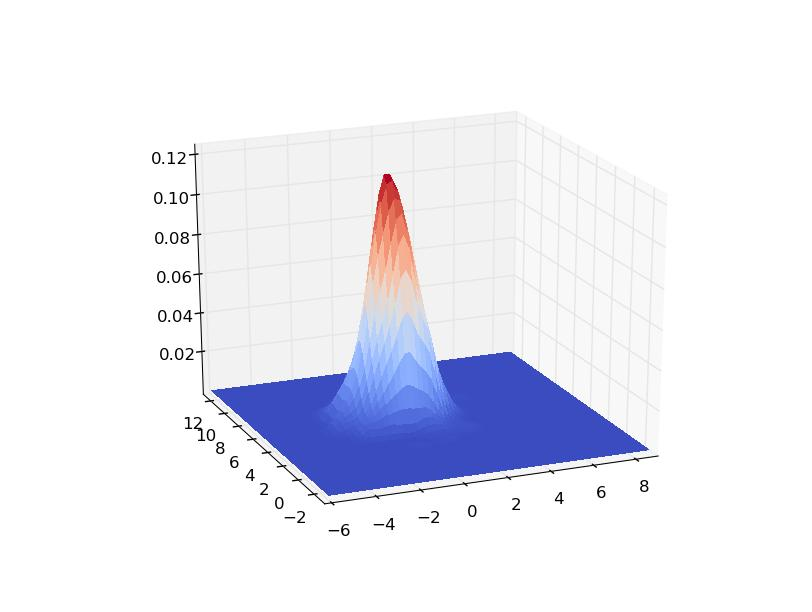
\includegraphics[width=\textwidth]{sum.jpeg}
		\caption{Sum of weighted multivariate normal random variables.}
	\end{subfigure}
	\begin{subfigure}[b]{.49\textwidth}
		\centering
		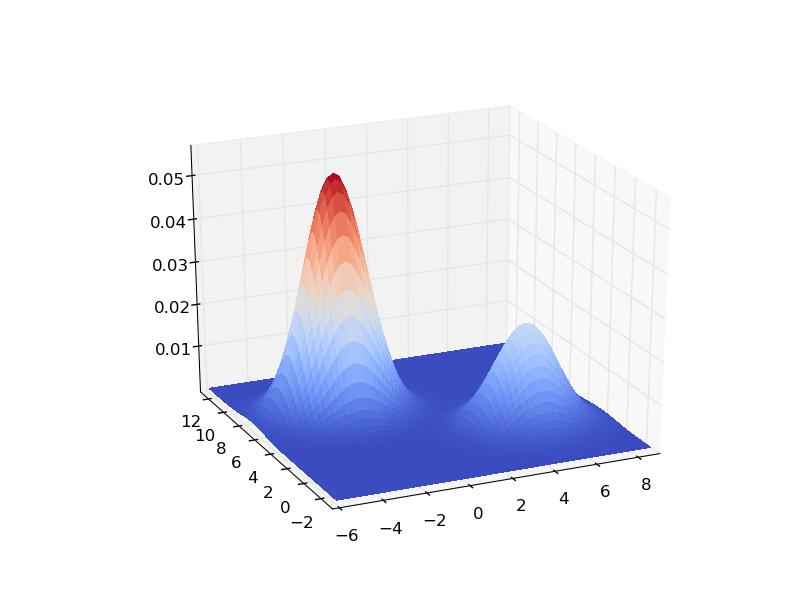
\includegraphics[width=\textwidth]{gmm.jpeg}
		\caption{Weighted mixture of multivariate normal random variables.}
	\end{subfigure}
	\label{threedplots}
\end{figure}

Thus, a fully defined GMM has parameters $\lambda = \left( w, \mathbf{\mu}, \mathbf{\Sigma} \right).$ The density of a GMM is given by $\mathbb{P}(x | \lambda) = \sum_{i=1}^{K} w_{i} \mathcal{N}(x ; \mu_{i}, \Sigma_{i})$ where
\begin{equation*}
\mathcal{N}(x ; \mu_{i}, \Sigma_{i}) = \frac{1}{(2\pi)^{\frac{K}{2}} |\Sigma_{i}|^{\frac{1}{2}}} e^{-\frac{1}{2} \left(x - \mu_{i} \right)^{T} \Sigma_{i}^{-1} \left(x - \mu_{i} \right)}
\end{equation*}

\begin{problem}
Write a function to evaluate the density of a normal distribution at a point $x$, given parameters $\mu$ and $\Sigma$. Include the option to return the log of this probability, but be sure to do it intelligently! Also write a function that computes the density of a GMM at a point $x$, given the parameters $\lambda$, along with the log option.
\end{problem}

Throughout this lab, we will build a GMM class with various methods. We will outline this now.

\begin{problem}
Write the skeleton of a GMM class. In the \li{\_\_init\_\_} method, it should accept the non-null parameter \emph{n\_components}, as well as parameters for the weights, means, and covariance matrices which define the GMM. Include a function to generate data from a fully defined GMM (you may use your code from the CDHMM lab for this), as well as the density function you recently defined.
\end{problem}

The main focus of this lab will be to estimate the parameters of a GMM, given observed multivariate data $Y = y_{1}, y_{2}, \cdots, y_{T}$. This can be done via Gibbs sampling, as well as with EM. We choose the latter approach for this lab. To do this, we must compute the probability of an observation being from each component of a GMM with parameters $\lambda^{(n)} = \left( w^{(n)}, \mu^{(n)}, \Sigma^{(n)}\right)$. This is simply 
\begin{equation*}
\mathbb{P}(x_{t} = i | y_{t}, \lambda) \propto w_{i}^{(n)} \mathcal{N}(y_{t} ; \mu_{i}^{(n)}, \Sigma_{i}^{(n)})
\end{equation*}
Just as with HMMs, we refer to these probabilities as $\gamma_{t}(i)$, and this is the \emph{E}-step in the algorithm. This might seem straightforward, except this direct computation will likely lead to numerical issues. Instead, we work in the log space, which means we have to be a bit more careful.

It is feasible (and occurs quite often) that each term $w_{i}^{(n)}\mathcal{N}(y_{t} ; \mu_{i}^{(n)}, \Sigma_{i}^{(n)})$ is $0$, because of underflow in the computation of the multivariate normal density. Letting $l_{i}^{(n)} = \ln w_{i}^{(n)} + \ln \mathcal{N}(y_{t} ; \mu_{i}^{(n)}, \Sigma_{i}^{(n)})$, we can compute these probabilities more carefully, as follows:
\begin{align*}
\mathbb{P}(x_{t} = i | y_{t}, \lambda) & = \frac{e^{l_{i}}}{\sum_{j=1}^{K} e^{l_{j}}} \\
& = \frac{e^{l_{i}}e^{-\max_{k} l_{k}}}{\sum_{j=1}^{K} e^{l_{j}}e^{-\max_{k} l_{k}}} \\
& = \frac{e^{l_{i} - \max_{k} l_{k}}}{\sum_{j=1}^{K} e^{l_{j} - \max_{k} l_{k}}}
\end{align*}
which will effectively avoid underflow problems.

\begin{problem}
Add a method to your class to compute $\gamma_{t}(i)$ for $t = 1, \cdots, T$ and $i = 1, \cdots, K$. Don't forget to do this intelligently to avoid underflow!
\end{problem}

Given our matrix $\gamma$, we can reestimate our weights, means, and covariance matrices as follows:
\begin{align*}
w_{i}^{(n+1)} & = \sum_{t=1}^{T} \gamma_{t}(i) \\
\mu_{i}^{(n+1)} & = \frac{\sum_{t=1}^{T} \gamma_{t}(i) y_{t}}{\sum_{t=1}^{T} \gamma_{t}(i)} \\
\Sigma_{i}^{(n+1)} & = \frac{\sum_{t=1}^{T} \gamma_{t}(i) (y_{t} - \mu_{i}^{(n+1)}) (y_{t} - \mu_{i}^{(n+1)})^{T}}{\sum_{t=1}^{T} \gamma_{t}(i)}
\end{align*}
for $i = 1, \cdots, K$. These updates are the \emph{M}-step in the algorithm.

\begin{problem}
Add methods to your class to update $w, \mu$ and $\Sigma$ as described above.
\end{problem}

With the above work, we are almost ready to complete our class. To train, we will randomly initialize our parameters $\lambda$, and then iteratively update them as above.

\begin{problem}
Add a method to initialize $\lambda$. Do this intelligently, i.e. your means should not be far from your actual data used for training, and your covariances should neither be too big nor too small. Your weights should roughly be equal, and still sum to $1$. Also add a method to train your model, as described previously, iterating until convergence within some tolerance.
\end{problem}

We will use our work to train the ``Mickey Mouse'' GMM, which has parameters
\begin{align*}
w & = \left[ \begin{array}{ccc} 0.7 & 0.15 & 0.15 \end{array} \right] \\
\mu_{1} & = \left[ \begin{array}{cc} 0.0 & 0.0 \end{array} \right] \\
\mu_{2} & = \left[ \begin{array}{cc} -1.5 & 2.0 \end{array} \right] \\
\mu_{3} & = \left[ \begin{array}{cc} 1.5 & 2.0 \end{array} \right] \\
\Sigma_{1} & = I_{3} \\
\Sigma_{2} & = 0.25 \cdot I_{3} \\
\Sigma_{3} & = 0.25 \cdot I_{3}
\end{align*}

To look at this GMM, we will evaluate the density at each point on a grid, as follows:
\begin{lstlisting}
>>> import matplotlib.pyplot as plt
>>> x = np.arange(-3, 3, 0.1)
>>> y = np.arange(-2, 3, 0.1)
>>> X, Y = np.meshgrid(x, y)
>>> N, M = X.shape
>>> immat = np.array([[model.dgmm(np.array([X[i,j],Y[i,j]])) for j in xrange(M)] for i in xrange(N)])
>>> plt.imshow(immat, origin=`lower')
>>> plt.show()
\end{lstlisting}

See Figure \ref{fig:mickeygmm} for this plot.
\begin{figure}[h]
\centering
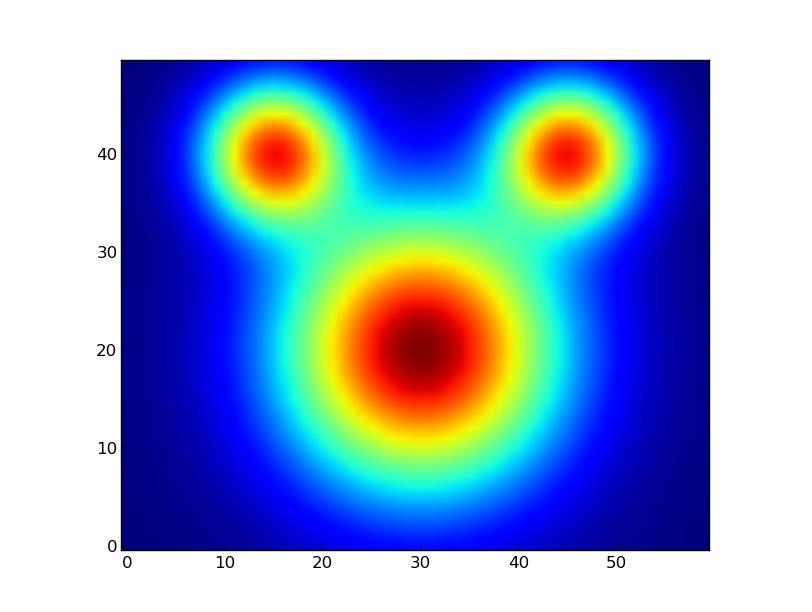
\includegraphics[width=\textwidth]{truemickeygmm.jpeg}
\caption{Density of true ``Mickey Mouse'' GMM.}
\label{fig:mickeygmm}
\end{figure}

\begin{problem}
Generate $750$ samples from the above mixture model. Using just the drawn samples, retrain your model. Evaluate and plot your density on the grid used above. How similar is your density to the original?
\end{problem}

How close is our trained model to the original one? We can use the symmetric Kullback-Liebler divergence to measure the distance between two probability distributions with densities $p(x)$ and $p'(x)$:
\begin{equation*}
SKL(p,p') = \abs{\frac{1}{2} \int p(x) \ln \frac{p(x)}{p'(x)} dx + \frac{1}{2} \int p'(x) \ln \frac{p'(x)}{p(x)} dx}
\end{equation*}

We cannot analytically compute this, so we use a Monte Carlo approximation, which uses the fact that 
\begin{equation*}
\frac{1}{N} \sum_{i=1}^{N} f(x_{i}) \rightarrow \int f(x) p(x) dx
\end{equation*}
as $N \rightarrow \infty$, assuming that each $x_{i} \sim p$. Then we have the following approximation of the symmetric KL divergence:
\begin{equation*}
SKL(p,p') \approx \frac{1}{2N} \abs{\sum_{i=1}^{N} \ln \frac{p(x_{i})}{p'(x_{i})} + \sum_{i=1}^{N} \ln \frac{p'(x_{i}')}{p(x_{i}')}}
\end{equation*}
where $x_{i} \sim p$ and $x_{i}' \sim p'$, for $N$ large.

\begin{problem}
Write a function to compute the approximate SKL of two GMMs. Compute the SKL between a randomly initialized GMM and the known GMM. Compute the SKL between the trained GMM and the known GMM. Is our trained model a good fit?
\end{problem}